\hypertarget{interfacejenes_1_1chromosome_1_1_allele_set_3_01_t_01_4}{
\section{jenes.chromosome.AlleleSet$<$ T $>$ Interface Reference}
\label{interfacejenes_1_1chromosome_1_1_allele_set_3_01_t_01_4}\index{jenes::chromosome::AlleleSet$<$ T $>$@{jenes::chromosome::AlleleSet$<$ T $>$}}
}
Inheritance diagram for jenes.chromosome.AlleleSet$<$ T $>$::\begin{figure}[H]
\begin{center}
\leavevmode
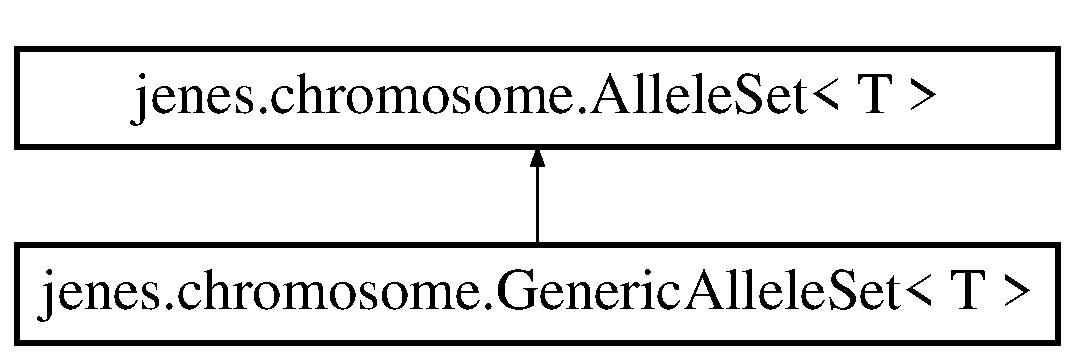
\includegraphics[height=2cm]{interfacejenes_1_1chromosome_1_1_allele_set_3_01_t_01_4}
\end{center}
\end{figure}
\subsection*{Public Member Functions}
\begin{CompactItemize}
\item 
abstract T \hyperlink{interfacejenes_1_1chromosome_1_1_allele_set_3_01_t_01_4_10625403643dc57a5c655a92a49aa644}{getElementAt} (int pos)
\item 
abstract T \hyperlink{interfacejenes_1_1chromosome_1_1_allele_set_3_01_t_01_4_c09d409c55d941892df658d21b3d4bff}{getRandomValue} ()
\item 
abstract int \hyperlink{interfacejenes_1_1chromosome_1_1_allele_set_3_01_t_01_4_3acbb10df92ebafc589d5d8546949f2f}{size} ()
\item 
abstract double \hyperlink{interfacejenes_1_1chromosome_1_1_allele_set_3_01_t_01_4_74ab0cb120fcfdee8e878727d6c50815}{difference} (T a0, T a1)
\end{CompactItemize}


\subsection{Detailed Description}
An AlleleSet represents an alphabet of object gene allele values. Each \hyperlink{}{ObjectChromosome.Gene} of an \hyperlink{classjenes_1_1chromosome_1_1_object_chromosome}{ObjectChromosome} has an allele set containing all the object values it can assume. A custom set of values can be determined by implementing this interface.

\begin{Desc}
\item[Parameters:]
\begin{description}
\item[{\em $<$T$>$}]class of elements held by AlleleSet\end{description}
\end{Desc}
\begin{Desc}
\item[Version:]2.0 \end{Desc}
\begin{Desc}
\item[Since:]1.0\end{Desc}
\begin{Desc}
\item[See also:]\hyperlink{classjenes_1_1chromosome_1_1_object_chromosome}{jenes.chromosome.ObjectChromosome} \end{Desc}


\subsection{Member Function Documentation}
\hypertarget{interfacejenes_1_1chromosome_1_1_allele_set_3_01_t_01_4_10625403643dc57a5c655a92a49aa644}{
\index{jenes::chromosome::AlleleSet$<$ T $>$@{jenes::chromosome::AlleleSet$<$ T $>$}!getElementAt@{getElementAt}}
\index{getElementAt@{getElementAt}!jenes::chromosome::AlleleSet< T >@{jenes::chromosome::AlleleSet$<$ T $>$}}
\subsubsection[getElementAt]{\setlength{\rightskip}{0pt plus 5cm}abstract T jenes.chromosome.AlleleSet$<$ T $>$.getElementAt (int {\em pos})\hspace{0.3cm}{\tt  \mbox{[}pure virtual\mbox{]}}}}
\label{interfacejenes_1_1chromosome_1_1_allele_set_3_01_t_01_4_10625403643dc57a5c655a92a49aa644}


Gets the allele value at the specified position 

\begin{Desc}
\item[Parameters:]
\begin{description}
\item[{\em pos}]the index of the desidered allele value \end{description}
\end{Desc}
\begin{Desc}
\item[Returns:]the allele value at the specified position \end{Desc}
\hypertarget{interfacejenes_1_1chromosome_1_1_allele_set_3_01_t_01_4_c09d409c55d941892df658d21b3d4bff}{
\index{jenes::chromosome::AlleleSet$<$ T $>$@{jenes::chromosome::AlleleSet$<$ T $>$}!getRandomValue@{getRandomValue}}
\index{getRandomValue@{getRandomValue}!jenes::chromosome::AlleleSet< T >@{jenes::chromosome::AlleleSet$<$ T $>$}}
\subsubsection[getRandomValue]{\setlength{\rightskip}{0pt plus 5cm}abstract T jenes.chromosome.AlleleSet$<$ T $>$.getRandomValue ()\hspace{0.3cm}{\tt  \mbox{[}pure virtual\mbox{]}}}}
\label{interfacejenes_1_1chromosome_1_1_allele_set_3_01_t_01_4_c09d409c55d941892df658d21b3d4bff}


Gets a random allele value within this alphabet. The allele value returned has to be a copy of the value in the allele set. 

\begin{Desc}
\item[Returns:]the random value selected \end{Desc}


Implemented in \hyperlink{classjenes_1_1chromosome_1_1_generic_allele_set_3_01_t_01_4_2f330d71d992e0d724bc31730b56229e}{jenes.chromosome.GenericAlleleSet$<$ T $>$}.\hypertarget{interfacejenes_1_1chromosome_1_1_allele_set_3_01_t_01_4_3acbb10df92ebafc589d5d8546949f2f}{
\index{jenes::chromosome::AlleleSet$<$ T $>$@{jenes::chromosome::AlleleSet$<$ T $>$}!size@{size}}
\index{size@{size}!jenes::chromosome::AlleleSet< T >@{jenes::chromosome::AlleleSet$<$ T $>$}}
\subsubsection[size]{\setlength{\rightskip}{0pt plus 5cm}abstract int jenes.chromosome.AlleleSet$<$ T $>$.size ()\hspace{0.3cm}{\tt  \mbox{[}pure virtual\mbox{]}}}}
\label{interfacejenes_1_1chromosome_1_1_allele_set_3_01_t_01_4_3acbb10df92ebafc589d5d8546949f2f}


Returns the alphabet size 

\begin{Desc}
\item[Returns:]the alphabet size \end{Desc}


Implemented in \hyperlink{classjenes_1_1chromosome_1_1_generic_allele_set_3_01_t_01_4_568ca617716496507d41e348c5bc2845}{jenes.chromosome.GenericAlleleSet$<$ T $>$}.\hypertarget{interfacejenes_1_1chromosome_1_1_allele_set_3_01_t_01_4_74ab0cb120fcfdee8e878727d6c50815}{
\index{jenes::chromosome::AlleleSet$<$ T $>$@{jenes::chromosome::AlleleSet$<$ T $>$}!difference@{difference}}
\index{difference@{difference}!jenes::chromosome::AlleleSet< T >@{jenes::chromosome::AlleleSet$<$ T $>$}}
\subsubsection[difference]{\setlength{\rightskip}{0pt plus 5cm}abstract double jenes.chromosome.AlleleSet$<$ T $>$.difference (T {\em a0}, \/  T {\em a1})\hspace{0.3cm}{\tt  \mbox{[}pure virtual\mbox{]}}}}
\label{interfacejenes_1_1chromosome_1_1_allele_set_3_01_t_01_4_74ab0cb120fcfdee8e878727d6c50815}


Provides the genetic difference between two alleles.

\begin{Desc}
\item[Parameters:]
\begin{description}
\item[{\em a0}]- first allele \item[{\em a1}]- second allele \end{description}
\end{Desc}
\begin{Desc}
\item[Returns:]- the genetic difeerence \end{Desc}


Implemented in \hyperlink{classjenes_1_1chromosome_1_1_generic_allele_set_3_01_t_01_4_ce70b10ee535ccc3a7cbcd42739b8d5c}{jenes.chromosome.GenericAlleleSet$<$ T $>$}.

The documentation for this interface was generated from the following file:\begin{CompactItemize}
\item 
src/jenes/chromosome/AlleleSet.java\end{CompactItemize}
